\section{V-Modell}
Das \textbf{V-Modell} (s. Abbildung~\ref{fig:v-modell}) wurde als Hilfestellung für analytische Maßnahmen entwickelt, um die im vorherigen Abschnitt erwähnten Maßnahmen in den Entwicklungsprozess zu integrieren (vgl.~\cite[10]{Wed09c}).

\begin{figure}
    \centering
    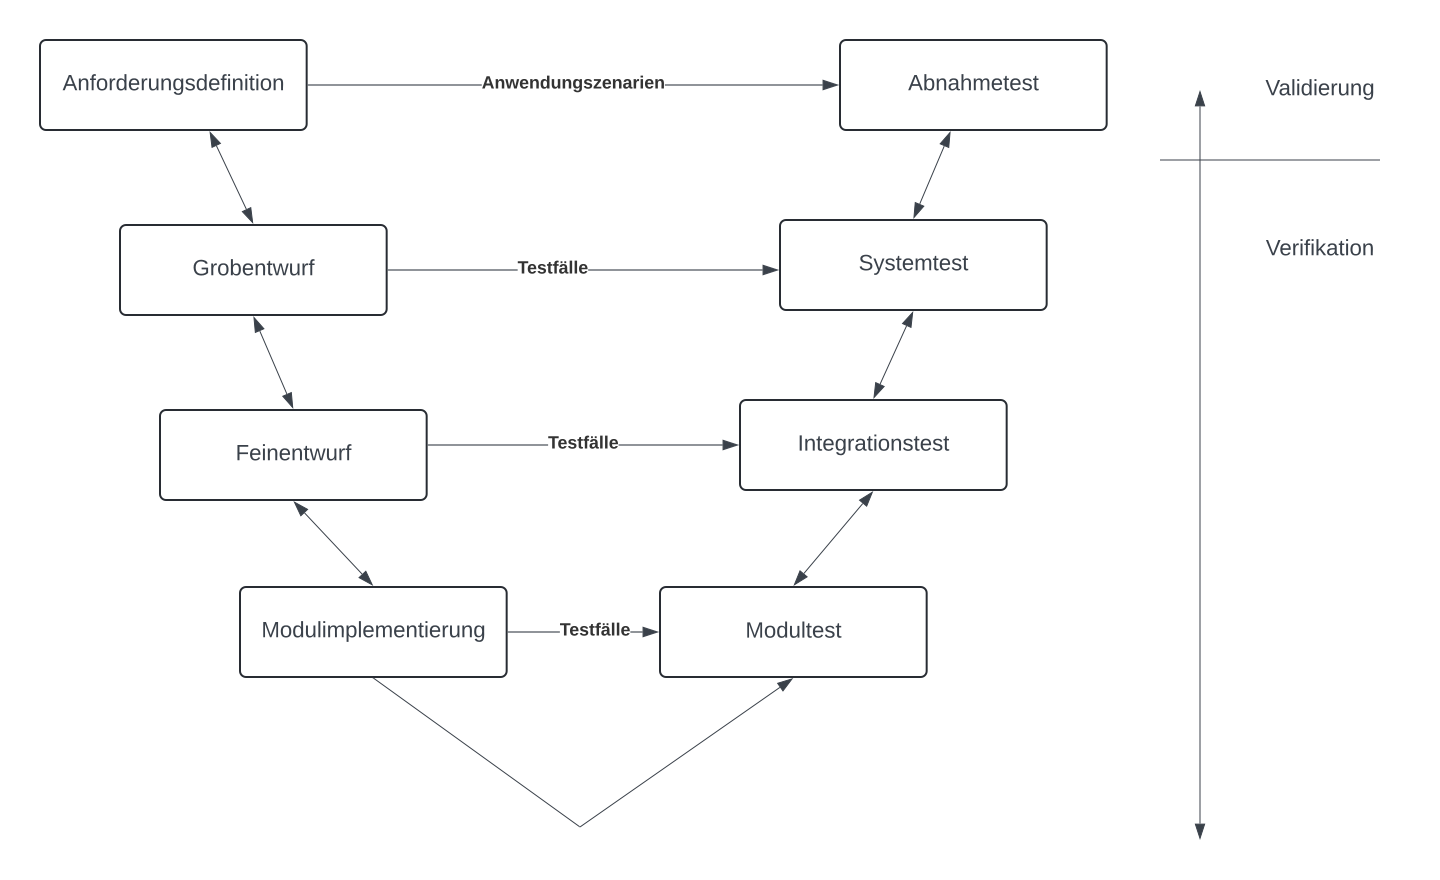
\includegraphics[scale=0.3]{chapters/Glossar/img/vmodell}
    \caption{Das Vorgehensmodell nach Boehm. (Quelle: in Anlehnung an \cite[554, Abb. 20.11-2]{Bal08})}
    \label{fig:v-modell}
\end{figure}

\noindent
Wie auf Abbildung~\ref{fig:v-modell} zu sehen ist stehen auf der linken Seite die bekannten Phasen des Wasserfallmodells.
Beim Übergang dieser Phasen werden die entstandenen Modelle oder Dokumente überprüft (\textit{Review}, die Übergänge werden auch als \textit{Qualitätstor} bezeichnet (vgl.~\cite[11]{Wed09c})), bevor mit der nächsten Phase begonnen wird.

\begin{itemize}
    \item Nach der \textbf{Realisierung} werden einzelne Klassen oder Module im Klassen- /Modultest getestet - dieser text wird auch \textbf{Komponententest} genannt.
    \item Danach werden die gestesteten Komponenten \textit{integriert} und gemeinsam getestet, was auf Basis des \textbf{Entwurfs} geschieht (\textbf{Integrationstests}).
    \item Nach der Integration wird das gesamte System in (möglichst) realer Umgebung getestet (\textbf{Systemtest} bzw. \textbf{Werkstest}).\\
    Grundlage für die Systemtests sind die Ergebnisse aus der Analyse.
    \item Im Anschluss wird das System  vom Kunden im \textbf{Abnahmetest} abgenommen, der auf Basis vertraglicher Vereinbarungen, also insb. der gemeinsam erarbeiteten \textbf{Anforderungen}, fußt
\end{itemize}

\subsection*{Verifikation und Validierung}
Die in diesem Zusammenhang verwendeten Begriffe \textbf{Verifikation} und \textbf{Validierung} haben folgende Bedeutung:

\begin{itemize}
    \item \textbf{Verifikation}: Es wird beurteilt, ob das als Resultat einer Entwicklungsphase vorliegende System bzw. die Komponenten den Vorgaben für diese Phase entsprechen (\textbf{Modul-} bis \textbf{Systemtest})
    \item \textbf{Validierung}: Es wird beurteilt, ob ein System oder eine Komponente während bzw. am Ende des Entwicklunsgprozesses die spezifizierten Anforderungen erfüllt (\textbf{Abnahmetest})
\end{itemize}

\subsection*{Inhalt der Testphasen}
Die \textbf{Modul-}, \textbf{Integrations-}, \textbf{System-} und \textbf{Abnahmetests}, beinhalten neben tests auch andere qualitätssichernde Maßnahmen:

\begin{itemize}
    \item \textbf{Modultest} beinhaltet neben dynamischen Tests auch werkzeuggestützte und manuelle Analysen
    \item \textbf{System-} bzw. \textbf{Integrationstests}: Es werden meistens nur Tests durchgeführt. Es finden aber auch Analysewerkzeuge ihren Einsatz, die bestimmte Qualitätsforderungen, wie z.B. die Wartbarkeit, global zu überprüfen
    \item \textbf{System-} bzw. \textbf{Abnahmetests} beinhalten manuelle Verfahren, bspw. zur Überprüfung von Handbüchern (Benutzerhilfen, Installationsanleitungen)
\end{itemize}

\subsection*{Tester}
\textbf{Integrations-} bzw. \textbf{Modultests} werden aus Gründen der Effizienz von den Entwicklern selber durchgeführt (auch: \textbf{Entwicklertests}, da die Entwickler die Fehler selber beheben können).\\
\textbf{Systemtests} werden i.d.R. von spezialisierten Testern durchgeführt.

\subsection*{Nützlichkeit des V-Modells}
Das V-Modell besitzt dieselben Probleme wie das \textbf{Wasserfallmodell}\footnote{
s. hierzu auch Abschnitt~\ref{sec:grenzen-des-wasserfallmodells}
}, da es eine Erweiterung bzw. Präzisierung des Wasserfallmodells darstellt (vgl.~\cite[12]{Wed09c}).\\
Allerdings ist es auch nützlich im Zusammenhang mit anderen Vorgehensmodellen (z.b. agilen Vorgehensmodellen): Insb. Modul- und INtegrationstests werden auch in iterativen Modellen während der Entwicklung genutzt, außerdem wird auch bei agilen Projekten vor Auslieferung noch eine Systemtestphase vorgeschaltet, und mit Abnahmetests sind Kunden in allen Fällen gut beraten.\\

\noindent
Es zeigt sich:

\blockquote[{\cite[12]{Wed09c}}]{
    Die Konzepte und Begriffe des V-Modells sind also von allgemeinerer Gültigkeit als das konkrete Vorgehen.
}